\documentclass[aspectratio=43]{beamer}
\usepackage[utf8]{inputenc}

%%%%%%%%%%%%%%%%%%%%%%%% THEME
\usetheme{material}
\useLightTheme
\usePrimaryPink
\useAccentIndigo

\usepackage{macros} % must come after theme

\title{\q Facts}
\keywords{\qc}

\begin{document}

\begin{frame}
	\titlepage
\end{frame}


\begin{frame}{Table of contents}
	\begin{card}
		\tableofcontents
	\end{card}
\end{frame}


\section{Introduction}
\begin{frame}{Introduction}
    \begin{card}
    This is an atypical week. Firstly, because it touches on various topics. Secondly, because these topics are \textit{typically} mentioned earlier when learning about quantum, but the author believes it ought to be easier to understand them at this point, some are also prerequisites for the upcoming content.\\
    So, some more considerations will be made on \textbf{\qcts}, namely universal gates, a new example of the consequences of unitary operators.\\ \textbf{Entanglement} will be explained, at last.\\ Finally, introductory notes on \textbf{Big O notation}.\\
    Thus: \q Facts!
    \end{card}
\pagenumber
\end{frame}

\section{Universal Gates}
\begin{frame}{Classical Universal Gates}
\begin{card}
    In \cc, any calculation is achievable through some simple sets of gates, for instance the set \{AND, NOT\} allows to derive any other operator. Moreover, there are singleton sets that also permit this, such as the \{NAND\} set (as a classical exercise you can try to simulate an OR using only NANDs).
\end{card}
\pagenumber
\end{frame}

\begin{frame}{\q Universal Gates}
\begin{card}
    After \qc (actually reversible computation came first) was initially thought of, and with the development of quantum gates, such simple sets were also procured. And they exist! Although they require some more complex considerations. We will not be proving this, as it is too theoretic and there are plenty of good explanations for it online, yet we will take a glimpse at what gates we would need.
\end{card}
\pagenumber
\end{frame}

\begin{frame}{\q Universal Gates}
\begin{cardTiny}
Firstly, it is \textbf{not} possible to do so using only single qubit operators (some we already know, others are here for completeness purposes):
    \begin{multicols}{2}
% $X = \begin{bmatrix}0 & 1\\ 1 & 0 \end{bmatrix}$
% $Y = \begin{bmatrix}0 & -i\\ i & 0 \end{bmatrix}$
% $Z = \begin{bmatrix}1 & 0\\ 0 & -1 \end{bmatrix}$
% $I = \begin{bmatrix}1 & 0\\ 0 & 1 \end{bmatrix}$
$T = \begin{bmatrix}1 & 0\\ 0 & \epsilon^{i\pi/4} \end{bmatrix}$
$S = \begin{bmatrix}1 & 0\\ 0 & i \end{bmatrix}$
$H = \begin{bmatrix}\osqrt  & \osqrt \\ \osqrt  & -\osqrt \end{bmatrix}$
    \end{multicols}
    \begin{equation*}
        \text{*Given: }\epsilon^{ix} = \cos(x) + i\sin(x)
    \end{equation*}
The first way of achieving the Universal Gate set is to take these single qubit gates and including the \textbf{CNOT} gate!
\end{cardTiny}
\pagenumber
\end{frame}

\begin{frame}{\q Universal Gates}
\begin{card}
The \textbf{Toffoli} (CCNOT) gate is one of the most eloquent gates that can perform any \textbf{Boolean} operation (universal for Boolean reversible computation). However, alone it is \textbf{not enough} for quantum universality. But, if we add to it the ability to \textbf{generate superposition}, with the \textbf{Hadamard} gate, they form a set of size two that is capable of quantum universal computation $\{Toffoli, H\}$. (There is another such pair $\{U_{qubit}, \sqrt{SWAP}\}$ which are gates you can research on your own). 
\end{card}
\pagenumber
\end{frame}

\begin{frame}{\q Universal Gates}
% \begin{cardTiny}
%     \small{Here's the Deutsch gate in extended form, you can probably see why it is hard to implement:}\\
%     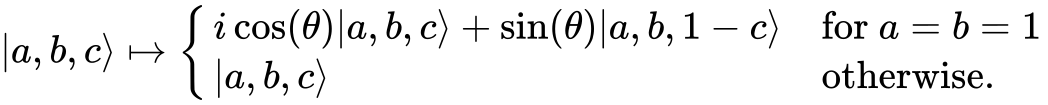
\includegraphics[width=0.7\textwidth]{deutsch}
% \end{cardTiny}
\begin{cardTiny}
\small{The Toffoli gate transformation maps 3 qubits and is therefore of size $2^3=8$. It is essentially an identity matrix, except for the intersection of the last two columns and two lines, which matches the X gate: \begin{bmatrix}0 & 1\\1 & 0\end{bmatrix} (Can you understand why?)}
\end{cardTiny}
\begin{cardTiny}
    \begin{multicols}{2}
    \small{This is the Toffoli gate in, you may notice some similarity with the CNOT gate, recall that this is also called CCNOT. The black circles actually represent both the control bits.}
    \begin{center}
        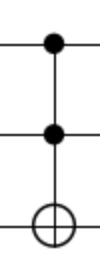
\includegraphics[width=0.3\textwidth]{toffoli} 
    \end{center}
    \end{multicols}
\end{cardTiny}
\pagenumber
\end{frame}



\section{Gates and Basis}
\begin{frame}{Gates and Basis}
    \begin{center}
        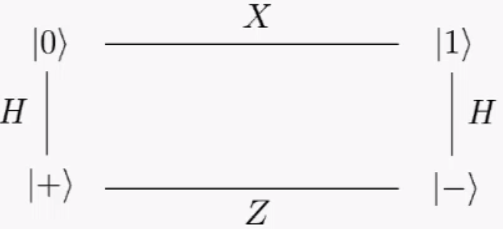
\includegraphics[width=0.6\textwidth]{basis_cycle} 
    \end{center}
    \begin{cardTiny}
        \small{The above diagram is a useful shorthand for quantum states conversion using quantum gates, and it also depicts the consequences of reversible computation. Literally, you can have a qubit in any of the four states $\ket{0},\ket{1},\ket{-}\ket{+}$ and obtain any other from it by performing simple one qubit gates.\\
        \textbf{Exercise:} Start with $\ket{0} = \begin{bmatrix}1 \\ 0\end{bmatrix}$ and obtain each of the other states by chaining the respective operations on this cycle.}
    \end{cardTiny}
\pagenumber
\end{frame}


\section{Entanglement}
\begin{frame}{Entanglement}
\begin{card}
    Entanglement is a curious phenomenon on a quantum level. It describes the state of a system in which the quantum state of two or more particles cannot be considered independently from each other. There is a correlation between their quantum properties. Pragmatically, if two qubits are entangled then measuring one will produce the measurement on the other to be the constant, when the experiment is repeated many times - they are entangled.\\ This property holds over long distances despite the uncertainty over the question we begin to be accustomed to: \textbf{Why?}
\end{card}
\pagenumber
\end{frame}

\begin{frame}{Entanglement possibilities}
\begin{cardTiny}
    This property carries both potential and controversy, as even Albert Einstein contested its possibility. Its existence is, however, unquestionable. We will not get into the paradoxical views and debate over different interpretations for it.
\end{cardTiny}
\begin{cardTiny}
    We will make use of it, and we actually already have, with the CNOT gate! Think about it: The state of a qubit \textbf{controls} the flipping of the other. In classical computing that would mean they are dependant, but in quantum terms they are entangled, \textbf{not just dependant}, because if we apply this gate to qubits in superposition, we get a non-deterministic result that is deterministically correlated.\\
    \small{This week's exercises will help understand entanglement.}
\end{cardTiny}
\pagenumber
\end{frame}

\section{Big O notation}
\begin{frame}{Big O notation}
\begin{card}
Lastly, on this factual menu, there comes a topic that most computer scientists already know, if this is your case, do not skip this slides, as some new concepts are introduced.
\end{card}
\begin{card}
Big O notation is used to describe the limiting behaviour of an algorithm (worst-case scenarios), essentially giving an estimate of the complexity (which reflects how the execution time evolves with the size of the input). 
\end{card}
\pagenumber
\end{frame}

\begin{frame}{Big O notation}
\begin{card}
The notation is as follows: $O(COMPLEXITY)$.\\
\begin{itemize}
    \item Assume you have a classical loop over an array of size $N$. The complexity of this algorithm in the Big O notation, would be $O(N)$.
    \item If you were to compute the square values of each cell in an $N\times N$ matrix, its complexity would be $O(N^2)$
    \item A typical \href{https://en.wikipedia.org/wiki/Binary_search_algorithm}{binary search} has a complexity of $O(log_2(N))$
\end{itemize}
\end{card}
\pagenumber
\end{frame}

\begin{frame}{Big O notation}
\begin{card}
    Computational problems are described by the most efficient algorithm that can solve them.\\ \p (polynomial) problems are classified as \textit{easy/efficiently solvable/tractable}, since the amount of time it takes to solve increasingly larger instances evolves polynomially.\\
    \np (nondeterministic polynomial time) problems, on the other hand, are not considered \textit{efficiently solvable}. This means that as the size of the problem instances increases linearly, the time (sometimes space) required grows exponentially. Nondeterministic implies not solvable on a deterministic \href{https://en.wikipedia.org/wiki/Turing_machine}{Turing Machines}.
\end{card}
\pagenumber
\end{frame}

\begin{frame}{Big O notation - \q impact}
\begin{card}[BQP]
    When we enter the \qw, and according to some advances we will study over this course, a new class of problems emerges: \bqp - bounded-error quantum polynomial time. This is a class of problems that is solvable in polynomial time in a \textbf{quantum computer} (with an error probability $\leq \frac{1}{3}$).
\end{card}
\pagenumber
\end{frame}

\begin{frame}{Big O notation - \q impact}
\begin{card}[NP vs BQP]
    The problem with this class is that it reflects the power of quantum computing, as some classical problems that belong to the \np class can be solved in \bqp. What is unclear is how far can quantum computers go, is \bqp a subset of \np or the other way around? do they match? Answering such questions would put a definite stamp on the power of \qc when compared with \cc.
\end{card}
\pagenumber
\end{frame}

\begin{frame}{Big O notation - \q impact}
\begin{center}
    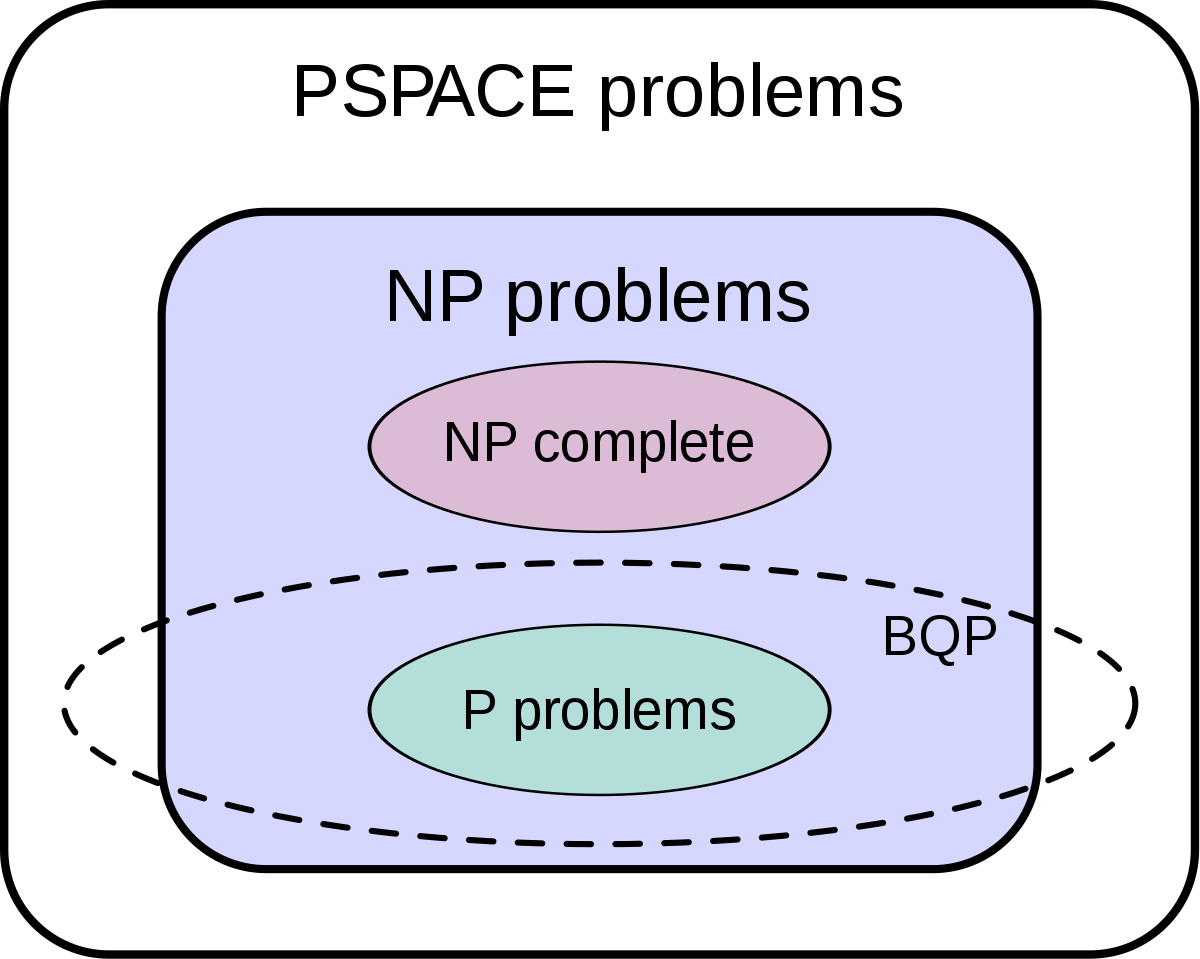
\includegraphics[width=0.8\textwidth]{bqp}
\end{center}
\pagenumber
\end{frame}

\begin{frame}{Exercises}
\begin{card}
When you are ready, you can head over to the \href{\weekFour/exercises/w4_01.ipynb}{exercises}, where the aforementioned concepts will be revised and where you will also learn some new concepts, such as \textbf{bell state}. Once you have finished, the \href{\weekFour/exercises/w4_01_s.ipynb}{solutions} contain detailed detailed explanation of what you should understand about the code you are developing!
\end{card}
\pagenumber
\end{frame}

\section{Where to learn more?}
\begin{frame}{Where to learn more?}
\begin{card}
    \begin{itemize}
    \item \href{http://www.drchinese.com/David/EPR.pdf}{The original Einstein–Podolsky–Rosen (EPR) paper}
    \item Medium article: \href{https://medium.com/quantum1net/einstein-and-entanglement-8c9f12e7f47b}{Einstein and entanglement}
    \item \href{https://en.wikipedia.org/wiki/Big_O_notation#Orders_of_common_functions}{Common computational complexities} with examples
    \item \href{https://en.wikipedia.org/wiki/P_versus_NP_problem}{P=NP?} major unsolved mathematical problem
    \end{itemize}
\end{card}
\end{frame}
\end{document}
